\documentclass{article}
\usepackage[utf8]{inputenc}
\usepackage{graphicx}
\graphicspath{ {./images/} }

\title{Rapport botTwitter}
\author{Gilbert Simon }
\date{May 2020}

\begin{document}

\maketitle

\section{Introduction}
The bot Twitter project is an react application which aim to enabl
e a user to easily create bot for twitter.
A user can create 2 type of bot. One is a "auto post" which will 
tweet with a time interval defined by the user
The other one, is a "response bot" will response to a mention with a defined message


\section{Team}
\begin{itemize}
    \item Simon Gilbert
    \item Ayoub Bhija
    \item AbdelHadim El Moutawakil
    \item Achraf Hanini
\end{itemize}

\section{A Bot}
A bot is a software application that is programmed to do certain tasks. Bots are automated, which means they run according to their instructions without a human user needing to start them up. Bots often imitate or replace a human user's behavior. Typically they do repetitive tasks, and they can do them much faster than human users could.
Bots usually operate over a network; more than half of Internet traffic is bots scanning content, interacting with webpages, chatting with users, or looking for attack targets. Some bots are useful, such as search engine bots that index content for search or customer service bots that help users. Other bots are "bad" and are programmed to break into user accounts, scan the web for contact information for sending spam, or perform other malicious activities

\section{Twitter}
Twitter is an online news and social networking site where people communicate in short messages called tweets.Twitter users follow other users. If you follow someone you can see their tweets in your twitter 'timeline'. 
Examples of most popular twitter's bots :
\begin{itemize}
\item@HundredZeros  is a Twitterbot that regularly tweets links to the eBooks that are free on Amazon
\item @DearAssistant is a an assistant like siri or google assisstant which try to answer your asks
\item@WhatTheFare is a uber bot and it give you the price for your ride uber when you tweet the adress of departure and the destination adress with the mention of the bot
\end{itemize}
\subsection{A Simulation}
This project is just a simulation of what we should get if we could access to the twitter API.
Sadly we didn't got a key so we couldn't use their API. We were restraint of simulate with json data
passed to some constant
We thought about using other API and other application but they rarely offer the same fonctionnality of twitter.
Mastodon, a clone decentralized of twitter was interesting but only one member knew it and even if it's open source, the decentralized aspect was a bit more complexe thant the centralized aspect of twitter

\section{Architecture Of the source code}
A react Project is typically based on the App.js which is the main file. 
\begin{itemize}
\item 	\textbf{App.js} is the main file and the first loaded
\item     \textbf{Twitter\_api.js} Contain all functions to call social network's Api.
\item 	\textbf{Components} Contain every component which build the application. This folder is dived      		into 2 folder, one for \textbf{Bot} and one for \textbf{Stats}. 
\item \begin{itemize}
    \item \textbf{Bot} This folder contains all components and views that permit the bot configuration
    \item \textbf{Stats} This folder contains all components and views that display the user informations
\end{itemize}

\item 	\textbf{Store} manage the store with \textbf{Redux} library, it's like a localDatabase
\item 	\textbf{assets}, This folder contain every assets like images
\end{itemize}

\section{Problems Encountered}
The First problem that we encountered is the time that we had to work on this project. During this period we were under pressure because we had many projects in parallel, specially the tutored project and the work company. The second problem encountered is the quarantine, it was a challenge to work together on a project remotely. The communication was reduced and every person of the group has his own planning, his tasks from his company. Finally we looked for many social network api that permit to manage an account, but unfortunately we don't found any free api's so to continue the development we choose the simulation.The simulation permit only to get Data but not to test automatic response and others features.

\section{Twitter Api Endpoints}
Here is some of the twitter api endpoints that we wanted to use :
\begin{itemize}
    \item To search a user : https://api.twitter.com/1.1/users/search.json
    \item To get folowers of a user : https://api.twitter.com/1.1/followers/list.json
    \item To search a tweet : https ://api.twitter.com/1.1/search/tweets.json
    \item To get tweets from a user : https://api.twitter.com/1.1/statuses/user\_timeline.json 
    \item To get tweets statistics : https://data-api.twitter.com/insights/engagement/\{stat\} 
\end{itemize}


\section{The applications}
\subsection{View to configure bots}
Simon tried to make the part about bot. So he made 2 different repository for each bot. One for the AutoPostBot and the other for the ResponseBot.
The creation of a bot will simply need a formulaire with a few informations, like the name of the bot, and the condition to make the bot work. For exemple, the time interval for the autoPostBot, or which word, or command, will activ the responseBot for getting the response
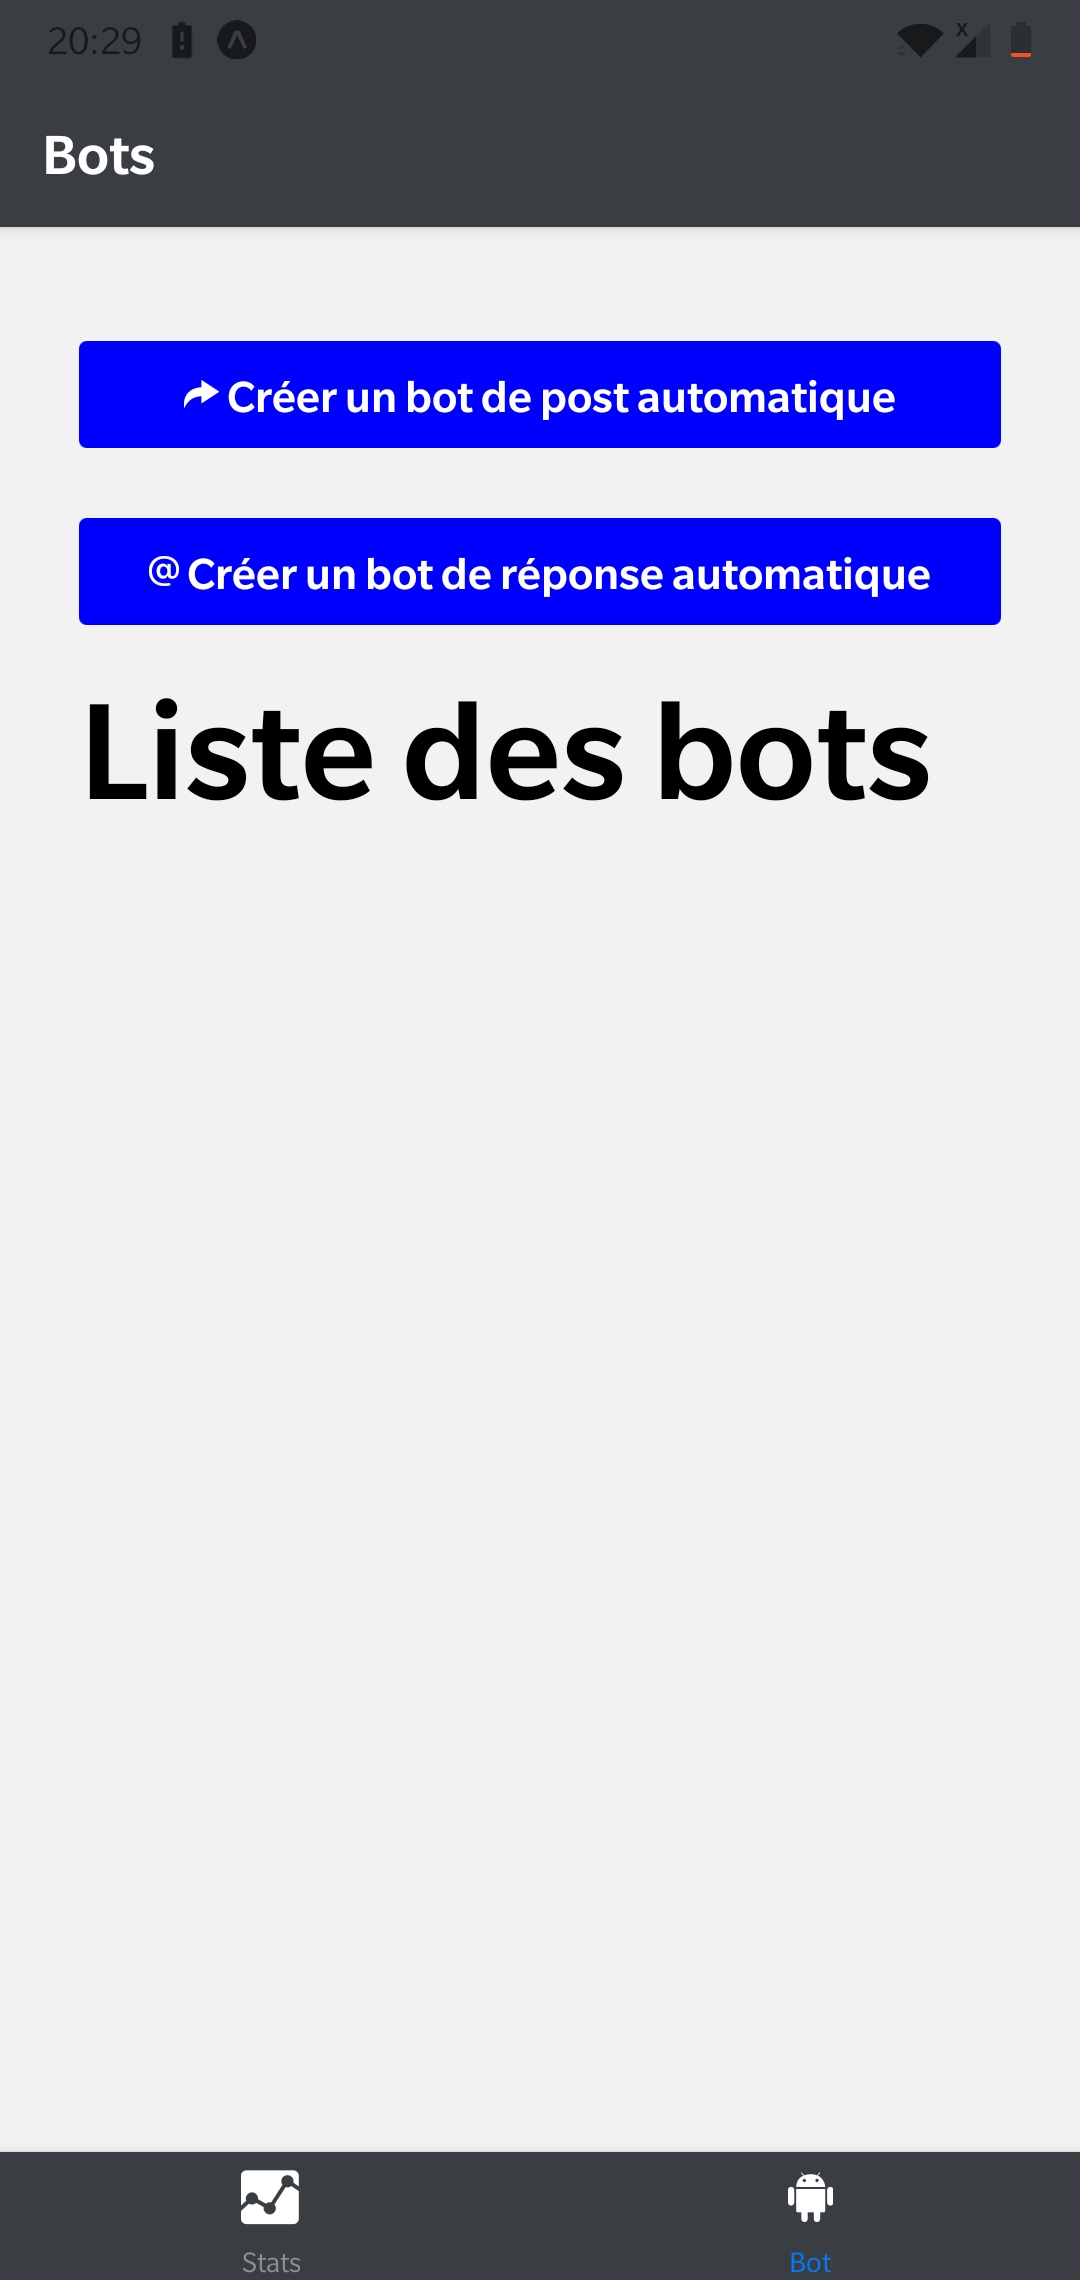
\includegraphics[height=1\textheight]{bots}
\subsection{View to configure users}
\includegraphics[height=1\textheight]{users and stats}
The part about fetching user and getting data was made by Simon. In the api file, a const is passed as a result. That mean that we will always get the same result. So we get a list of 2 user, after that we can select a user to see more informations like how many tweet he did, how many follower he have or how many account does he follow.


\section{Conclusion}
This project is very interesting because it permit to see many notions that are important today in a mobile project like the external api's. The use of external api's is today the most used technique to persist data and use it from different platform like web apps, mobiles app, desktop apps. It was a challenge to work on this project due to many events. We know that we haven't finished and completed the features but we wanted to show thought this report the differents encountered problems and solutions envisaged.
The use of an API is a fundamental to know in programmation, and this project manly based on this functionality was useful for our own skil.
It open our view to make new app or project like for exemple, a react peer application
\end{document}

